% outline

% title-me
% EBCWA problem
% ideal solution (solution attributes)
% DITA (verse fail http://media.boreme.com/post_media/2008/tank-toll.jpg)
% docutils (nearly success)
%  MS-Word -> docbookXML -> reST
%  recognise verses (1saiah)
%  verse role
%  biblepassage directive
%  document linking/sharing
%  draft-comment
% sphinx
%  conf.py
%  toctree
%  4 types (all html, 1 pdf, 1 epub, 1 google-docs) (bible-version, draft)
% paver
%  paver <type> book <version> <draft> <force>
%  override conf.py with cog
%  run pdflatex with rubber
%  singlehtml->insert css with cog->google-doc

\newcommand{\rst}{reStructuredText}
\documentclass{beamer}
\usepackage{minted}
\usetheme{default}
\hypersetup{colorlinks=true}
\usepackage{framed}

\title{TheoreST: Publishing Theology with Python}
\author{Carl Cerecke}
\institute{Evangelical Bible College of Western Australia}
\date{September 8, 2013}

\begin{document}

    \begin{frame}[plain]
        \titlepage
    \end{frame}

    \begin{frame}{Overview of the talk}
        \begin{itemize}
        \item Problem (and ideal solution)
        \item A tank is not the solution
        \item Proprietary format $\rightarrow$ \rst
        \item \rst $\rightarrow$ web/pdf/epub
            \begin{itemize}
            \item docutils
            \item sphinx
            \end{itemize}
        \item Automating with \texttt{paver}
        \item Other tools/technologies
        \item Todo\ldots
        \end{itemize}
    \end{frame}
    
    \begin{frame}{The problem}
        \begin{itemize}
        \item ~300 books in MS Word format (written over 20+ years)
            \begin{itemize}
            \item Systematic Theology
            \item Pastoral Theology
            \item Commentaries
            \item Miscellaneous topics 
            \end{itemize}
        \item Distribute as widely and conveniently as possible
        \item ``Freely you have been given, freely give''
        \end{itemize}
    \end{frame}
    
    \begin{frame}{The (ideal) solution}
        \begin{itemize}
        \item One authoritative source, multiple outputs
        \item Share common document fragments
        \item Bible version independent
        \item Bible references hyperlinked: \href{http://some.url}{John 3:16}
        \item Build individual books (pdf/epub), or whole collection (html)
    \end{itemize}
\end{frame}
    
\begin{frame}
    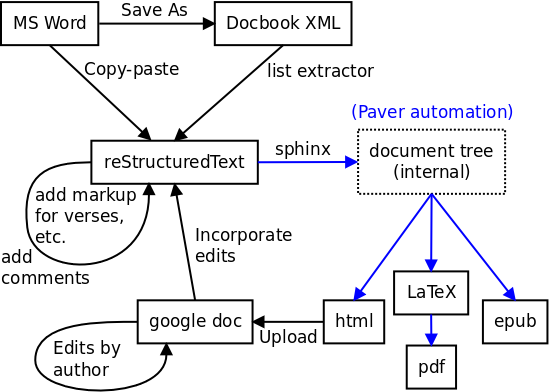
\includegraphics[keepaspectratio=true, width=\paperwidth]{theorest_process.png}
\end{frame}
    
    \begin{frame}{DITA: the Wrong Way}
        \begin{itemize}
        \item DITA: Enterprise-level technical documentation
        \item XML
        \item Java
        \item Deal-breaker: Too static.\\
            Dynamically determine bible-reference URLs during document creation?
        \end{itemize}
    \end{frame}
    
    \begin{frame}[plain]
        \centerline{
\includegraphics[keepaspectratio=true, width=\paperwidth]{tank-toll.jpg}}
    \end{frame}
    
    \begin{frame}{\rst markup language (PEP 287)}
        Put example here\\
        include roles and directives
    \end{frame}

    \begin{frame}{MS Word format to \rst}
        
\includegraphics[keepaspectratio=true, width=\paperwidth]{typewriter_keyboard.jpg}
    \end{frame}
    
    \begin{frame}{MS Word problems}
    No styles\\
        Enumerated lists
        \begin{framed} %{enumerated lists}
            \ldots\\
3. EVALUATION\\
\quad (a) Persecuted in Damascus; escapes in basket (Acts 9:20-25)\\
\quad (b) Driven out of Jerusalem, sent to Tarsus (Acts 9:28-30).\\
\quad (c) Stoned at Lystra and thought to have died (Acts 14:19).\\
        \quad (d) Paul whipped and imprisoned at Phillipi (Acts 16:16-24).\\
        \ldots
    \end{framed}
    Solution:\\
    \emph{Save As...} docbook XML format. Guess indent level.  
    \end{frame}
    
    \begin{frame}[fragile]
        \frametitle{Recognising bible references}
         Want to replace:\\
         \begin{verbatim}Lorem ipsum John 3:16 dolor
\end{verbatim}
         with:\\
         \begin{verbatim}Lorem ipsum `John 3:16` dolor
\end{verbatim}
Other examples:
\begin{itemize}
\item multiple verses: John 3:16,20
\item verse range: John 3:16-20
\item whole chapter: John 3
\item Multi chapter: John 3:16, 4:4
\item Multi book, chapter, verse, range:\\
    John 3:16-18,20,4:1, 3 John 1:2, Luke 1:1
\end{itemize}
\end{frame}

\begin{frame}
    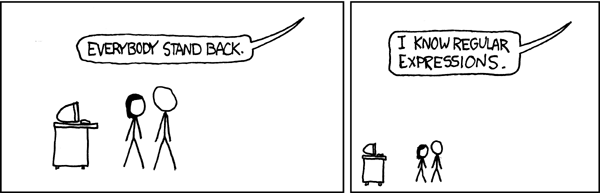
\includegraphics[keepaspectratio=true, width=0.9\paperwidth]{regular_expressions.png}
\end{frame}

\begin{frame}[fragile]
    
\begin{minted}{python}
names = ['Genesis', 'Exodus', ..., 'Revelation']
re_names = '('+'|'.join(names)+')'
re_raw = '('+re_names+r'\s+\d+:(\s*(,|-|;|:|'+\
    re_names+'|\d+))+'+')'
re_bibref = re.compile(re_raw)

def bibquote(text):
    return re_bibref.sub(r'`\1`', text)
\end{minted}

What about lsaiah? or I Corinthians?

\end{frame}

\begin{frame}[fragile]{Parsing the verse roles}
Need to translate `John 3:16-18,20` into:

\begin{minted}{html}
<a href="http://bible.xyz/ESV/john3+3:16-18">
John 3:16-18</a>,
<a href="http://bible.xyz/ESV/john3+3:20">20</a>
\end{minted}

Actually, internal document-tree nodes representing links.

\end{frame}

\begin{frame}[fragile]{Tokenisation}
Use python's own tokeniser

\begin{minted}{bash}
> echo "John 3:16-18,20" | python3 -m tokenize
1,0-1,4:            NAME           'John'         
1,5-1,6:            NUMBER         '3'            
1,6-1,7:            OP             ':'            
1,7-1,9:            NUMBER         '16'           
1,9-1,10:           OP             '-'            
1,10-1,12:          NUMBER         '18'           
1,12-1,13:          OP             ','            
1,13-1,15:          NUMBER         '20'           
1,15-1,16:          NEWLINE        '\n'           
2,0-2,0:            ENDMARKER      ''             
\end{minted}

\end{frame}

\begin{frame}[fragile]{Parsing}

\begin{itemize}
\item Plenty of parser-generators available.

\item Too heavyweight.

\item Verse references don't nest.

\item But do need lookahead:
\begin{minted}{python}
'John' '3' ':' '16' '-' '18' ',' '20' ...
\end{minted}

\item Solution: Use a state machine

\pause
\item Problem: No goto :-(

\pause
\item Solution: My goto function decorator:\\
\url{http://code.activestate.com/recipes/576944-the-goto-decorator/}

\pause
\item Problem: Only python 2
\end{itemize}
\end{frame}

\begin{frame}[fragile]{Parsing state machine}

One method per state.

Each method-state returns next method-state

\begin{minted}{python}
def parse(self):
    ...
    state = self.p_book            # start state
    while state:
        state = state()
		
def p_book(self):                  # expecting a book
    self.book = self.swallow(Book) # exception if not Book
    self.text += self.book.value   # collect link text
    return self.p_chapter          # 'goto' this state
	
def p_chapter(self):               # expecting a chapter
    ...
\end{minted}
\end{frame}

\begin{frame}{Adding verse role to sphinx}
\end{frame}

\begin{frame}{Automating the build process}
Problem: minimise effort to build documentation

What I want to build:
\begin{itemize}
\item All documents in integrated sphinx website
\item Individual documents as pdf/epub/html-for-google-docs
\end{itemize}
For each build I want to specify:
\begin{itemize}
\item bible version (ESV, KJV, NET, etc.)
\item 'draft' (include comments?)
\end{itemize}

Solution: paver

\end{frame}

\begin{frame}{Automating the build process with paver}
"Paver is a Python-based build/distribution/deployment 
scripting tool along the lines of Make"

What I want:
\begin{itemize}
\item paver command here
\end{itemize}

\end{frame}

\begin{frame}[fragile]{Multiple build files for sphinx?}


\begin{minted}{python}
a=b

def parse(foo):
    bar.baz
\end{minted}
\end{frame}

\begin{frame}{Future work}
\begin{itemize}
\item Robust versioning scheme
\end{itemize}

\end{frame}
\end{document}
